%!TEX ROOT=main.tex
\chapter{Software}
Tato kapitola se zaměří na popis připojených jednotek ze softwarového hlediska.
\begin{figure}[H]
    \label{fig:sw_diagram}
    \caption{Digram připojených periférii k MCU}
    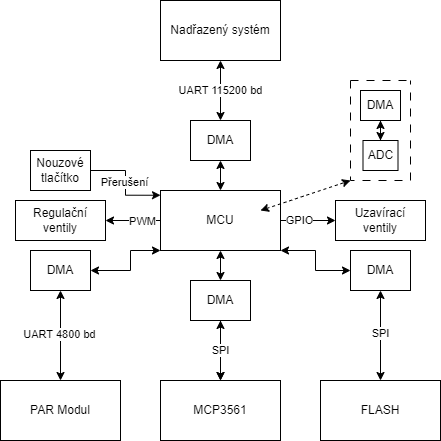
\includegraphics[width=1\textwidth]{pictures/sw_diagram.png}
\end{figure}
MCU STM32F407ZG6 je postaveno na architektůře Arm Cortex M4 s přidaným jádrem a instrukcemi pro výpočty plouvoucích čísel.
Programování MCU probíha v programovacím prostředí od ST Micro. STM32CubeIDE, které má v sobě zabudovaný kompilátor, prostředí pro debuggina a prostředky pro nahrání SW do MCU.
\begin{figure}[H]
    \caption{Ukázka vývojového prostředí STM32CubeIDE pro mikroprocesory STM32}
    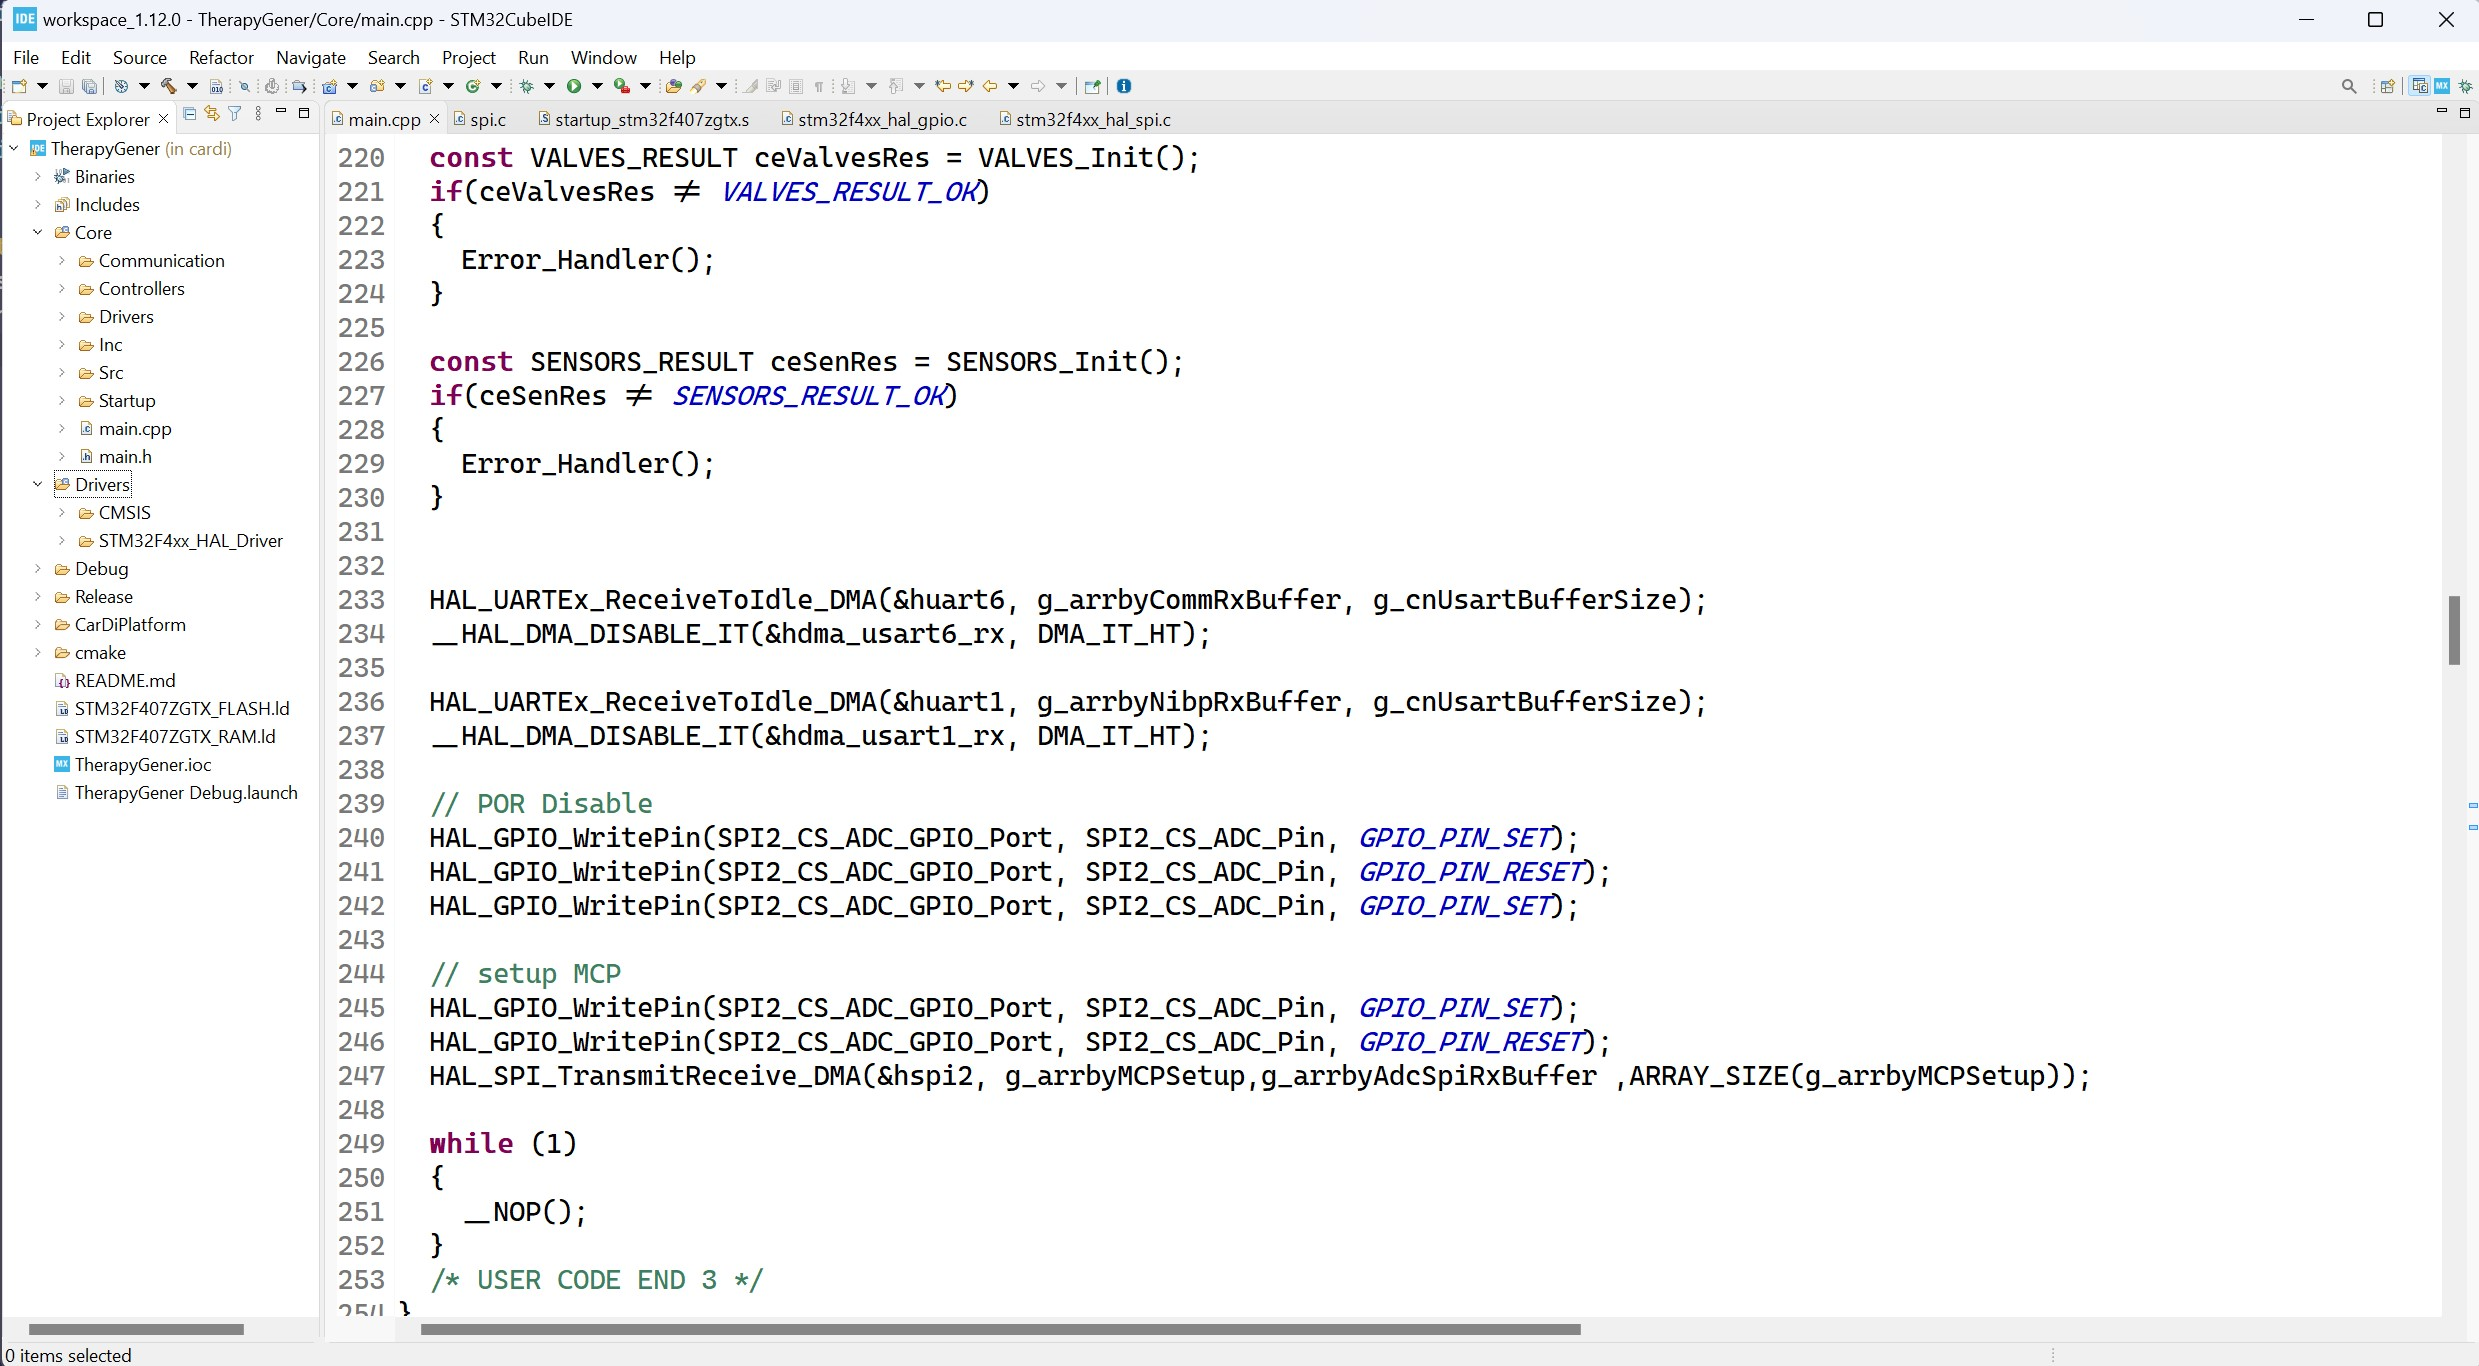
\includegraphics[width=1\textwidth]{pictures/cubeide.jpg}
\end{figure}
STM32CubeIDE také sprostředkovává ovladače pro komunikaci s internímy periferiemy a prostředí pro konfiguraci MCU.
\begin{figure}[H]
    \caption{Konfigurace GPIO pinů MCU}
    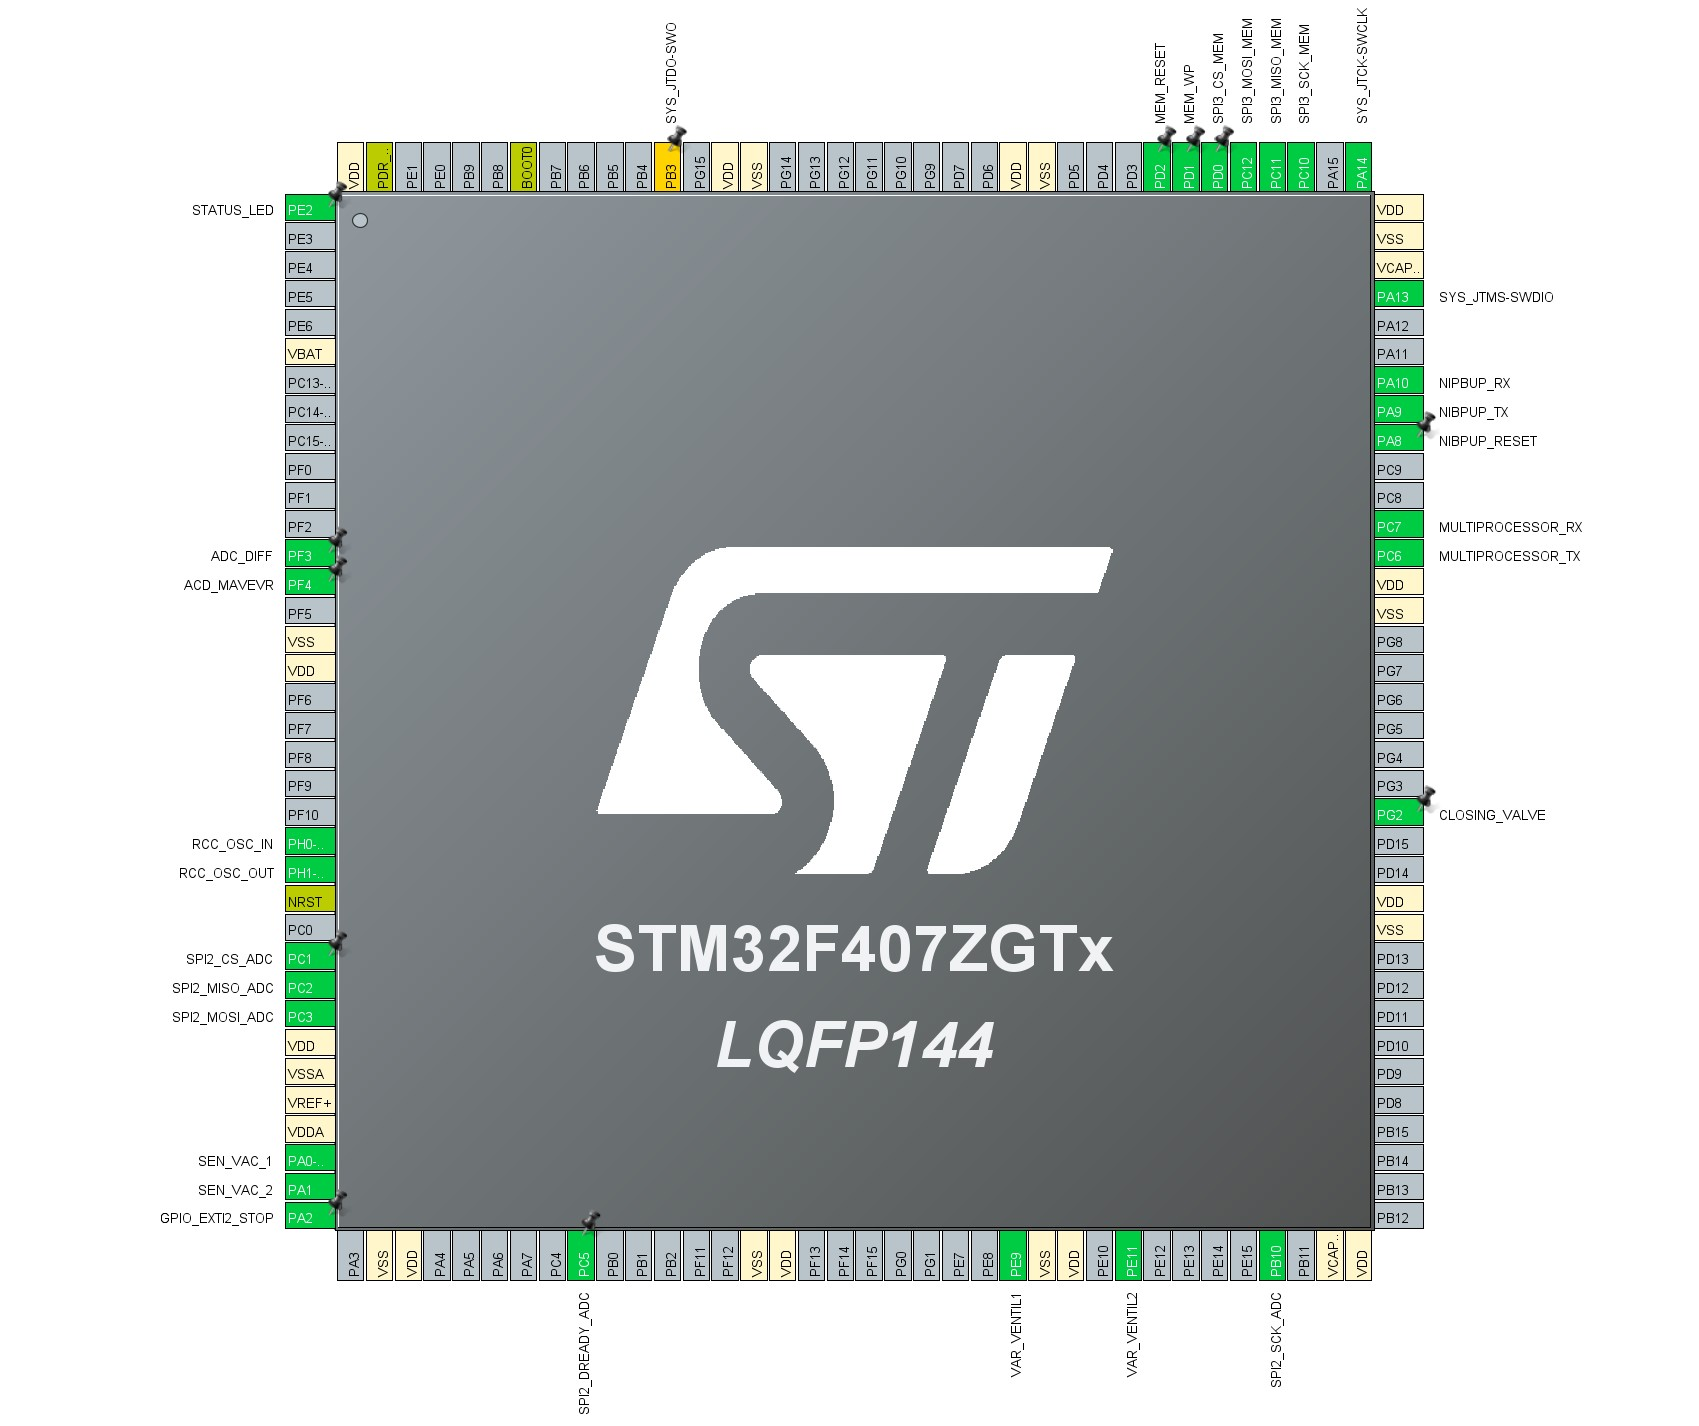
\includegraphics[width=0.8\textwidth]{pictures/mcu_settings.jpg}
\end{figure}
Po zvolení konfigurace MCU STM32CubeIDE samo vygeneruje základní softwarovou inicializaci periférií.
